% Slides — Capítulo 8: Satélites e Radar
\documentclass[aspectratio=169,11pt]{beamer}
\usepackage{../comum/temameteo}
\graphicspath{{../figuras/cap08/}}

\title[Cap. 8 --- Satélites e Radar]{Capítulo 8 --- Satélites e Radar}
\subtitle{Meteorologia Prática}
\author{}
\date{}

\begin{document}

\begin{frame}
  \titlepage
  \vfill
  \atribuicao
\end{frame}

\begin{frame}{Roteiro}
  \tableofcontents
\end{frame}

% ---------------------------------------------------------------
\section{Órbitas}

\begin{frame}{Geoestacionária: Newton no quadro}
  \begin{columns}
    \column{0.44\textwidth}
    \eqdestaque{$\dfrac{GM}{r^2} = \omega^2 r \Rightarrow
      r = \left(\dfrac{GM}{\omega^2}\right)^{1/3}$}
    \vspace{0.4em}
    \begin{itemize}
      \item $T = $ dia \alert{sideral} (86164\,s) $\Rightarrow$
            $z = 35\,790$\,km.
      \item GOES/Meteosat/Himawari: filme contínuo de um hemisfério.
      \item Sem cobertura polar; resolução $\sim$km.
    \end{itemize}
    \column{0.56\textwidth}
    \figlivroslide{fig_08_14.jpg}{0.5\textheight}{Fig.~8.14 --- órbita
      heliosíncrona acompanhando o Sol ao longo do ano}
  \end{columns}
\end{frame}

\begin{frame}{Polar heliosíncrona: o varredor global}
  \begin{columns}
    \column{0.44\textwidth}
    \begin{itemize}
      \item $\sim$850\,km, $T \simeq 102$\,min: globo inteiro
            2$\times$/dia, na \alert{mesma hora solar local}.
      \item O achatamento da Terra precessa a órbita $360°$/ano — de
            graça.
      \item Resolução fina; base dos sondadores e da assimilação
            (Cap.~20).
    \end{itemize}
    \column{0.56\textwidth}
    \figlivroslide{fig_08_12.jpg}{0.5\textheight}{Fig.~8.12 --- órbita
      polar: a Terra gira embaixo da trilha}
  \end{columns}
\end{frame}

% ---------------------------------------------------------------
\section{Funções peso: o satélite sondador}

\begin{frame}{De que altura vem o sinal?}
  \begin{columns}
    \column{0.44\textwidth}
    \eqdestaque{$W(z) = \dfrac{d\tau}{dz} = k\rho(z)\,\tau(z)$}
    \vspace{0.4em}
    \begin{itemize}
      \item ``Ter emissor'' ($k\rho$) × ``conseguir escapar''
            ($\tau$).
      \item Pico na profundidade óptica $=1$ (T2).
      \item Canal mais absorvente $\Rightarrow$ enxerga mais alto.
    \end{itemize}
    \column{0.56\textwidth}
    \begin{center}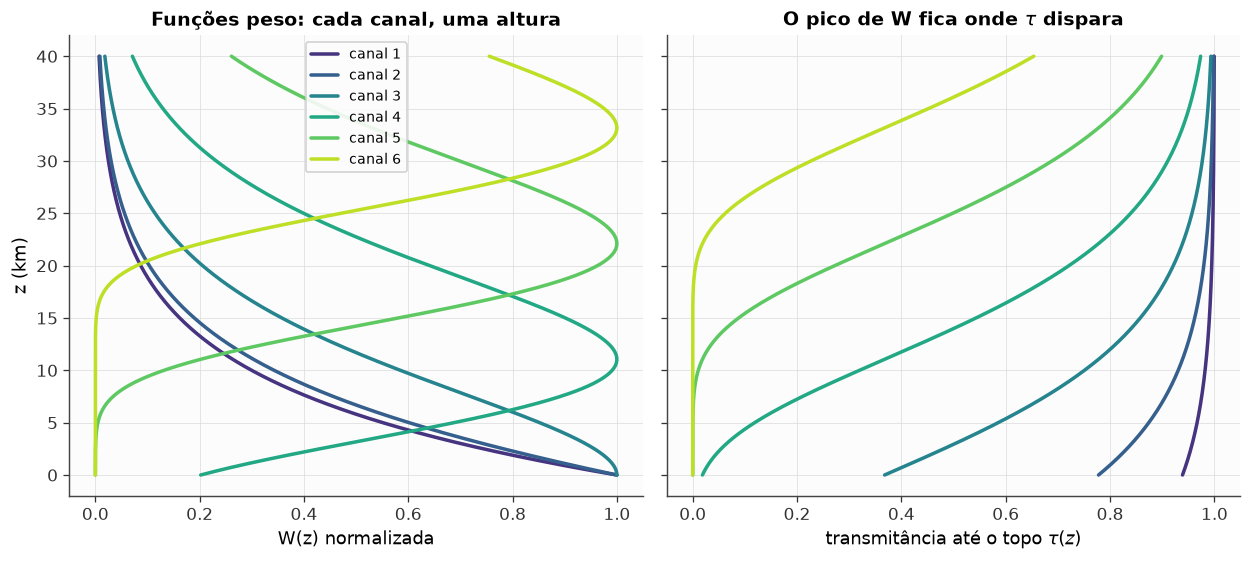
\includegraphics[width=\linewidth]{notebook_funcoes_peso.png}\\[-2pt]
    {\tiny funções peso e transmitância — Caso~2 do notebook do curso}\end{center}
  \end{columns}
\end{frame}

\begin{frame}{Os canais reais de um sondador}
  \begin{columns}
    \column{0.4\textwidth}
    \begin{itemize}
      \item GOES: cada canal IR com $W$ picando numa altura — a
            atmosfera fatiada em camadas.
      \item Inversão radiância $\to$ $T(z)$: problema mal-posto, os
            $W$ se sobrepõem — nasce a assimilação variacional
            (Cap.~20).
      \item É assim que o globo inteiro tem ``sondagem'' sem balão.
    \end{itemize}
    \column{0.6\textwidth}
    \figlivroref{Fig.~8.11}{funções peso dos canais do sondador GOES}{2017 EUMETSAT}
  \end{columns}
\end{frame}

\begin{frame}{As janelas e as bandas}
  \begin{columns}
    \column{0.4\textwidth}
    \begin{itemize}
      \item Janelas ($\tau \approx 1$): o satélite vê o chão — canal
            IV 10{,}7\,$\mu$m (Cap.~2).
      \item Bandas de absorção: H$_2$O 6{,}7\,$\mu$m, CO$_2$
            15\,$\mu$m — vê o \alert{ar}, de propósito.
      \item ``Janela suja'': aerossol e continuum contaminam.
    \end{itemize}
    \column{0.6\textwidth}
    \figlivroslide{fig_08_3.jpg}{0.5\textheight}{Fig.~8.3 ---
      transmitância espectral: janelas e bandas de absorção}
  \end{columns}
\end{frame}

% ---------------------------------------------------------------
\section{Interpretando imagens}

\begin{frame}{Visível × IV × vapor}
  \centering
  \begin{tabular}{lll}
    \hline
    Canal & mede & leitura \\
    \hline
    visível (0{,}6\,$\mu$m) & luz refletida & \alert{brilhante $=$
    espessa} \\
    IV janela (10{,}7\,$\mu$m) & $\sigma T^4$ do topo & \alert{frio $=$
    alta} \\
    vapor (6{,}7\,$\mu$m) & H$_2$O média/alta & umidade mesmo sem nuvem \\
    \hline
  \end{tabular}
  \vspace{0.6em}
  \begin{itemize}
    \item Combinações: brilhante$+$frio $=$ Cb; brilhante$+$quente $=$
          estrato; escuro$+$frio $=$ cirrus.
    \item Escuro no vapor $=$ ar seco descendente — as intrusões dos
          ciclones (Cap.~13).
    \item $T_B \to$ altura do topo com a atmosfera padrão (T3, Cap.~1).
  \end{itemize}
\end{frame}

\begin{frame}{As mesmas nuvens em dois canais}
  \begin{columns}
    \column{0.3\textwidth}
    \begin{itemize}
      \item Compare: estratos brilham no visível mas somem no IV
            (topo quente).
      \item Cirrus fino: quase invisível no visível, frio no IV.
      \item Caso~1 do notebook treina a classificação.
    \end{itemize}
    \column{0.35\textwidth}
    \figlivroref{Fig.~8.16a}{canal visível}{SSEC, Univ. of Wisconsin}
    \column{0.35\textwidth}
    \figlivroref{Fig.~8.16d}{canal infravermelho}{SSEC, Univ. of Wisconsin}
  \end{columns}
\end{frame}

% ---------------------------------------------------------------
\section{Radar: eco, $Z$ e chuva}

\begin{frame}{A geometria da varredura}
  \begin{columns}
    \column{0.4\textwidth}
    \begin{itemize}
      \item Pulso $\lambda\sim5$--10\,cm; alcance $R = c\Delta t/2$.
      \item Varredura cônica (PPI) em vários ângulos $\to$ volume 3-D
            a cada $\sim$5\,min.
      \item Feixe sobe com a distância: a 200\,km olha $\sim$3\,km de
            altura — perde chuva rasa.
    \end{itemize}
    \column{0.3\textwidth}
    \figlivroslide{fig_08_24a.jpg}{0.4\textheight}{Fig.~8.24 --- PPI:
      varredura cônica}
    \column{0.3\textwidth}
    \figlivroslide{fig_08_28a.jpg}{0.4\textheight}{Fig.~8.28 --- altura
      do feixe vs.\ distância}
  \end{columns}
\end{frame}

\begin{frame}{Refletividade e a relação $Z$--$R$}
  \begin{columns}
    \column{0.44\textwidth}
    \eqdestaque{$Z = \sum D^6$;\quad dBZ $= 10\log_{10}Z$;\quad
      $Z = aR^b$}
    \vspace{0.4em}
    \begin{itemize}
      \item $D^6$: Rayleigh — o radar adora gotas grandes (Cap.~7).
      \item 20\,dBZ chuvisco $\cdot$ 40\,dBZ $\sim$10\,mm/h $\cdot$
            55$+$ granizo.
      \item $\pm3$\,dB $\Rightarrow$ $+60/-40\%$ em $R$ (T5): radar
            precisa de pluviômetro.
    \end{itemize}
    \column{0.56\textwidth}
    \figlivroslide{fig_08_28b.jpg}{0.52\textheight}{Fig.~8.28 ---
      classificação operacional de intensidade por dBZ}
  \end{columns}
\end{frame}

\begin{frame}{Armadilhas de leitura}
  \begin{columns}
    \column{0.44\textwidth}
    \begin{itemize}
      \item \alert{Banda brilhante}: anel de neve derretendo — água
            veste o floco e infla $Z$ (Cap.~7).
      \item Atenuação (banda X): a tempestade da frente apaga a de
            trás (Beer, Cap.~2).
      \item Ecos de terreno e propagação anômala em inversões
            (Cap.~5).
    \end{itemize}
    \column{0.56\textwidth}
    \figlivroslide{fig_08_29.jpg}{0.5\textheight}{Fig.~8.29 --- a banda
      brilhante no nível de derretimento}
  \end{columns}
\end{frame}

% ---------------------------------------------------------------
\section{Doppler}

\begin{frame}{O dilema do Doppler}
  \begin{columns}
    \column{0.5\textwidth}
    \eqdestaque{$R_{max} = \dfrac{c}{2\mathrm{PRF}}$,\quad
      $V_{max} = \dfrac{\lambda\,\mathrm{PRF}}{4}
      \Rightarrow R_{max}V_{max} = \dfrac{c\lambda}{8}$}
    \vspace{0.4em}
    \begin{itemize}
      \item Fase entre pulsos $\to$ $V_r$ (radial apenas).
      \item Alcance longo × velocidade alta: \alert{inimigos}.
      \item $|V| > V_{max}$ dobra (\emph{aliasing}) — Caso~4 simula e
            corrige.
    \end{itemize}
    \column{0.5\textwidth}
    \figlivroslide{fig_08_33.jpg}{0.46\textheight}{Fig.~8.33 --- fase
      entre pulsos sucessivos: a medida Doppler}
  \end{columns}
\end{frame}

\begin{frame}{Assinaturas Doppler que salvam vidas}
  \begin{columns}
    \column{0.34\textwidth}
    \begin{itemize}
      \item Rotação (mesociclone): dipolo vermelho/verde
            \alert{perpendicular} ao feixe (Cap.~15).
      \item Divergência (downburst): dipolo \alert{alinhado} ao feixe
            (Cap.~14).
      \item Polarização dual: forma — chuva × granizo × insetos.
    \end{itemize}
    \column{0.33\textwidth}
    \figlivroslide{fig_08_38b.jpg}{0.42\textheight}{Fig.~8.38 ---
      assinatura de tornado/mesociclone}
    \column{0.33\textwidth}
    \figlivroslide{fig_08_38c.jpg}{0.42\textheight}{Fig.~8.38 ---
      assinatura de downburst}
  \end{columns}
\end{frame}

% ---------------------------------------------------------------
\section{Síntese e laboratório}

\begin{frame}{O mapa do capítulo}
  \eqdestaque{$r = (GM/\omega^2)^{1/3} \;\to\; W = d\tau/dz \;\to\;
    Z = \Sigma D^6,\ Z = aR^b \;\to\; R_{max}V_{max} = c\lambda/8$}
  \vspace{0.6em}
  Órbitas levam os olhos ao lugar certo; funções peso fatiam a
  atmosfera; $Z$--$R$ transforma eco em chuva; Doppler acrescenta o
  vento — com um dilema embutido.
\end{frame}

\begin{frame}{Laboratório numérico --- notebook do Cap.~8}
  \texttt{notebooks/cap08\_sensoriamento.ipynb}
  \begin{enumerate}
    \item Órbitas: período e cobertura vs.\ altitude.
    \item Funções peso: o sondador de 6 canais.
    \item $Z$--$R$: inversão, ruído e divergência entre relações.
    \item Aliasing Doppler e um dealias por continuidade.
  \end{enumerate}
  \vspace{0.4em}
  \textbf{Exercícios}: T1--T5 e N1--N4 nas notas; células reservadas no
  notebook.
  \vfill
  \atribuicao
\end{frame}

\end{document}
